\section{Uparivanje značajki (engl. feature matching)}

Nakon što se odrede SIFT značajke na obije slike, potrebno je pronaći podudaranja među njima. Proces se svodi na pronalaženje parova deskriptora koji su međusobno najsličniji u visokodimenzionalnom prostoru. Postoji nekoliko metoda za mjerenje sličnosti deskriptora.

Prva metoda je korištenje \textit{brute force} algoritma. Sličnost između dva 128-dimenzionalna SIFT deskriptora mjeri se koristeći Euklidsku udaljenost formulom
\begin{equation}
    d(d_1, d_2) = \sqrt{\sum_{i=1}^{128} (d_1[i] - d_2[i])^2}
\end{equation}
gdje su $d_1$ i $d_2$ dva 128-dimenzionalna SIFT deskriptora. Manja Euklidska udaljenost predstavlja veću sličnost između deskriptora, odnosno između lokalnih struktura slike koje oni predstavljaju.
Kada bi se uparivanje izvodilo jednostavnim pronalaskom para sa minimalnom udaljenosti došlo bi do velikog broja pogrešnih podudaranja. Zbog toga se koristi algoritam zvan Loweov test omjera~\cite{lowe2004sift}. Umjesto da se traži samo jedan, za svaki deskriptor s referentne slike pronalaze se dva najbliža susjeda na slici s kamere. Ako je omjer udaljenosti između najbližeg i drugog najbližeg susjeda manji od koeficijenta $t$, deskriptor se smatra valjanim podudaranjem. Ovo se može opisati formulom
\begin{equation}
    \frac{d(d_1, d_2)}{d(d_1, d_3)} < t
\end{equation}
gdje su $d_1$, $d_2$ i $d_3$ tri 128-dimenzionalna SIFT deskriptora, $d$ je Euklidska udaljenost, a $t$ je koeficijent koji se koristi za filtriranje pogrešnih podudaranja. Uobičajena vrijednost za prag $t$ je između 0.7 i 0.8. Ovaj test provjerava je li podudaranost nedvosmislena, odnosno ako je najbliži susjed znatno bliži od drugog onda je značajka jedistvena i podudarnost je vjerojatno ispravna. Ako to nije istina onda to ukazuje na dvosmislenost i takva podudaranost se odbacuje kao nepouzdana.

Unatoč što ovaj algoritam daje dobre rezultate, njegova vremenska komplesnost ga čini nepraktičnim za rad u stvarnom vremenu. Kako bi se ubrzao proces, često se koriste algoritmi za aproksimativnu pretragu najbližih susjeda koji se oslanjaju na efikasne strukture podataka za organizaciju visokodimezionalnih vektora. 
Jedna od takvih struktura je \textit{k-d stablo}. K-d stablo je prostorna podatkovna struktura koja rekurzivno dijeli prostor u polovične podprostore čime postiže brzu eliminaciju velikih dijelova prostora pretrage. Unatoč njenoj efikasnosti u prostorima niske dimenzionalnosti, njena primjena u visokodimenzionalnim prostorima nije učinkovita, što je problematično za 128-dimenzionalne SIFT deskriptore. 
Zato je za SIFT deskriptore bolja tehnika LSH (eng. \textit{Locality-Sensitive Hashing}) koja se oslanja na hash funkcije za brzo pronalaženje sličnih vektora u visokodimenzionalnom prostoru.
U praksi se takvi algoritmi ne implementiraju ručno već se koriste gotove biblioteke koje nude bolja rješenja. Jedna od takvih biblioteka je \textit{FLANN} (eng. \textit{Fast Library for Approximate Nearest Neighbors}) koja implementira više različitih algoritama, uključujući i k-d stablo i LSH~\cite{flannmatcher}. Bitno je navesti kako u sklopu \textit{OpenCV} implementacije FLANN-a nije moguće koristiti LSH algoritam za uparivanje SIFT značajki jer je LSH algoritam implementiran samo za binarne deskriptore.
Prednost FLANN-a je u tome što može automatski odabrati najprikladniju strukturu podataka i parametre pretrage na temelju podataka i odabranih kompromisa brzine ili preciznosti. Tim algoritmima i bibliotekama se postižu veće brzine uz minimalne gubitke u preciznosti naspram \textit{brute force} algoritma.

\begin{figure}[H]
    \centering
    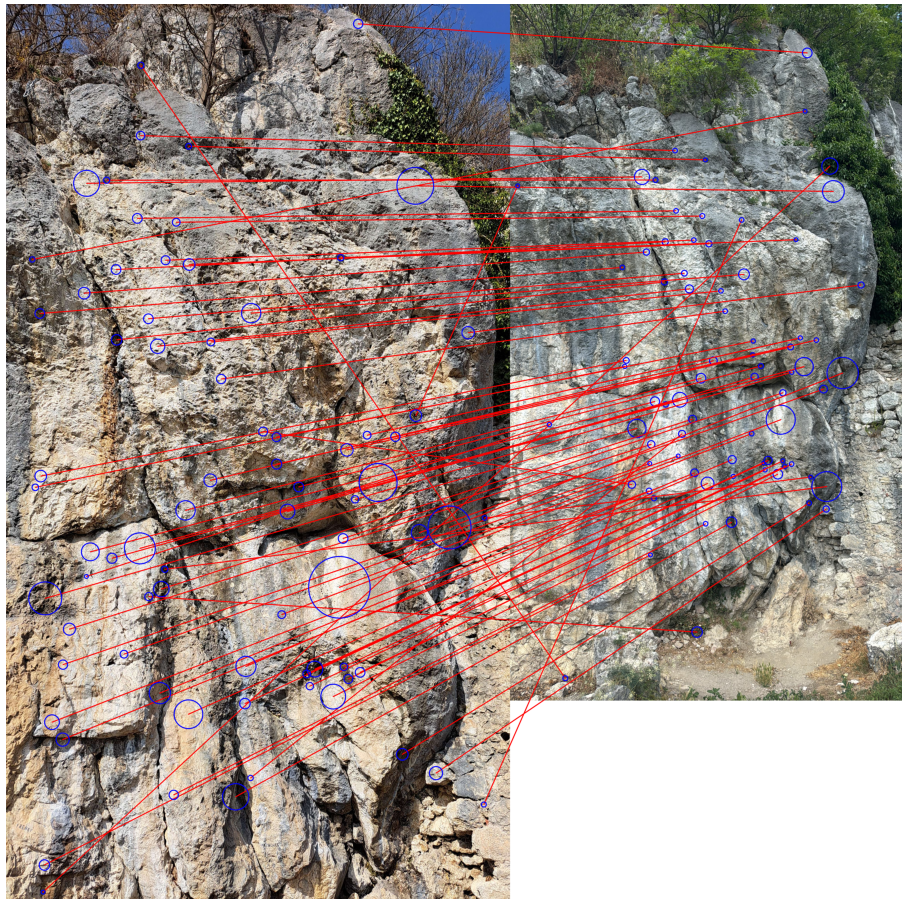
\includegraphics[width=0.9\textwidth]{images/racunalniVid/feature_matching.png}
    \caption{Uparivanje značajki SIFT algoritmom}
    \label{fig:uparivanje_znacajki}
\end{figure}

Na slici~\ref{fig:uparivanje_znacajki} prikazan je primjer uparivanja značajki SIFT algoritmom za referentnu sliku penjačkog smjera i sliku dobivenu s kamere mobilnog uređaja.